% !TEX encoding = UTF-8
% !TEX TS-program = pdflatex
% !TEX root = ../main.tex
% !TEX spellcheck = en-EN

%************************************************



Deep learning is showing very effective and promising results in a number of areas, often surpassing those obtained with the old methods. In this chapter we will show
how we apply deep learning techniques to plant phenotyping, in particular we will show how the network used is adapted to different plants and how it can extrapolate
individual leaves from the images.

\section{Our Method}
Segment each instance of a plant is an hard work, images can have different dimension, and each plant can have different position in an image. For this reason, we decided
to identify each plant separately and then go on to identify each instance. In order to classify each plant, we made use of different technologies and we needed to modify
the datasets at our disposal. To do this we used an online tool called Make Sense, which allowed us to create the position annotations of the boxes for object detection.

\section{Object Detection}
For the development of object detection of individual plants we used one of the best known and most powerful neural networks in the field of object detection YOLO
\cite{redmon2016look}. This network, taken in version 5, in contrast to the sliding windows, sees the entire image during training and test time so it implicitly encodes
contextual information about classes as well as their appearance. Inside YOLO the separate components of object detection are unified into a single neural network.
It divides the input image into an $S \times S$ grid. If the center of an object falls into a grid cell, that grid cell is responsible for detecting that object.
Each grid cell predicts B bounding boxes and confidence scores for those boxes. Each of this consists of 5 predictions: x, y, w, h, and confidence. The (x, y)
coordinates represent the center of the box relative to the bounds of the grid cell. The width and height are predicted relative to the whole image. Finally
the confidence prediction represents the IOU between the predicted box and any ground truth box.
\begin{figure}[h]
    \centering
    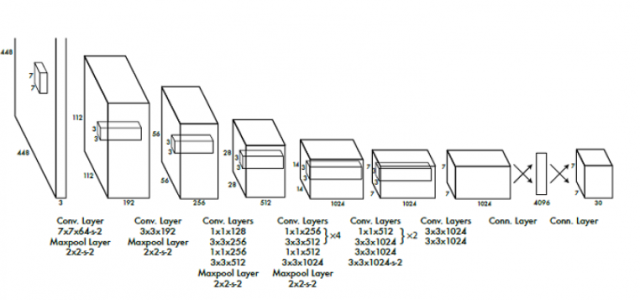
\includegraphics[width=1\textwidth]{yolo_net} 
    \caption{YOLO architecture}
\end{figure}
YOLO is inspired by GoogLeNet \cite{Szegedy_2015_CVPR} model for image classification, it has 24 convolutional layers followed by 2 fully connected layers.
Instead of the inception modules used by GoogLeNet, YOLO simply use $1 \times 1$ reduction layers followed by $3 \times 3$ convolutional layers.

At the end of the training, we used YOLO in such a way as to obtain the individual plants from each image containing different quantities from our dataset. Several
frames are then created, one for each plant identified by the network, which are then placed in a folder and catalogued in two files, one containing the data in COCO
\cite{lin2014microsoft} format, where all the images created are listed, while the second file contains information regarding the position (x, y) in the original image
of the plant just cut out. All this has been created to facilitate the adaptation to the segmentation network and to recompose the data.


\section{Instance Segmentation}
The instance segmentation part is performed by BlendMask \cite{chen2020blendmask}. Here we use this convnet in order to segment each instance of leaves. All the leaves found
are saved into a file with the segmentation map still in COCO format. This convnet is a hybrid of top-down and bottom-up approaches, BlendMask consists of a detector
network and a mask branch. The mask branch has three parts, a bottom module to predict the score maps, a top layer to predict the instance
attentions, and a blender module to merge the scores with attentions. 

\begin{figure}[h]
    \centering
    \includegraphics[width=1\textwidth]{blendmask_net} 
    \caption{Blendmask pipeline, }
\end{figure}

The bottom module predicting score maps which that are called bases. The input for the bottom module could be backbone features like YOLACT or Panoptic FPN. 
Into the top layer the authors append a single convolution layer on each of the detection towers to predict top-level attentions. Then the blender module get as input the 
bottom-level bases, where with a RoIPooler in Mask R-CNN crops the bases with each proposal, and the it resize the region to a fixed size.
During training, the net simply use ground truth boxes as the proposals. During inference, FCOS \cite{tian2019fcos} predict the results. 

Thanks to this network, we achieved good results in leaf detection and segmentation, so we figured out how to implement the next section that extrapolate the information about
the leaves. 




\section{Feature extraction}
After segmentation we collect the information about the extracted leaf and derive only those with a probability of not being covered greater than 80\%.
Next, we save the predictions coming out of the blendmask in a file containing both the leaf identifier and the name of the image to which the leaf belongs.
With this, we are able to find out where the leaf is present in the image, so that in the next step we can extrapolate it from the depth image. In this way, we will
finally obtain the 3D image with an rgb part and the fourth dimension, which is the depth. By means of a simple remapping we then obtain the xyz position on the camera plane.
$$
\begin{cases}
    Z = z / depth_scale \\
    X = (x - cx) * Z / fx \\
    Y = (y - cy) * Z / fy
\end{cases}
$$
Here we have two camera intrinsics which can be used to compute this functions. Those are related to the image which we are refferring to. $cx$, $cy$, $fx$ and $fy$ are the 
center of camera image and the $f$ are the focal length of the lens. Now with the xyz positions of the image we can finally calculate the various properties. The first
most interesting one will be the area of the leaf for which we will rely on the pyvista library, otherwise for the calculation of the major and minor axes we will make
use of the scikit-learn library. We also calculated the height of the intrinsic leaf and the height of the leaf from the ground so that we could see how high it is from
the ground and how high it actually is.





\section{Other Networks}
In order to understand which network was best for our purpose, we used different CNNs, so that we could understand which one was best suited to different types of leaves
in different contexts.


\subsection{YOLACT}
The first network used was YOLACT (You Only Look At CoefficienTs) \cite{bolya2019yolact}. The network proposes to split instance segmentation into two simpler tasks,
first it generates a non-local prototype mask dictionary for the entire image, then it predicts a linear combination of coefficients per instance. Thus, producing
a full-image instance segmentation from these two components is straightforward: for each instance, linearly combine the prototypes using the corresponding
predicted coefficients and then crop with a predicted bounding box. We show that by segmenting in this way, the network learns to locate instance masks on its own,
where visually, spatially and semantically similar instances appear different in the prototype. This approach also has several practical advantages.
First and foremost, it’s fast: because of its parallel structure and extremely lightweight assembly process, YOLACT adds only a marginal amount of computational overhead to
a one-stage backbone detector, making it easy to reach 30 fps even when using ResNet-101. Secondly, the masks are of high quality: since the masks use the full extent of
the image space without any loss of quality from repooling, these masks for large objects turn out to be of significantly higher quality than those of other methods.

YOLACT is composed of different components, the backbone formed by the resnet, is the one used for the classification of the objects present in the scene.
It is flanked by the Feature Pyramid Network (FPN) suitably modified to obtain a more precise classification and, where the softmax cross entropy is used to refine
the prediction process.

\begin{figure}[h]
    \centering
    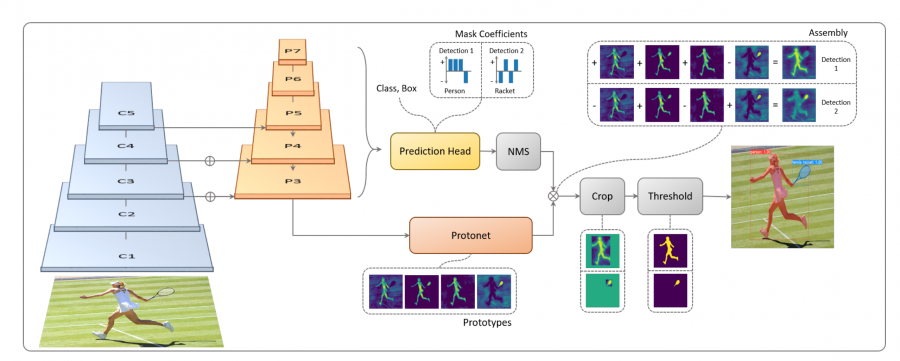
\includegraphics[width=1\textwidth]{yolact_net} 
    \caption{YOLACT model using ResNet-101 + FPN}
\end{figure}

The prototype generation branch (protonet) predicts a set of k prototype masks for the entire image. The authors implemented this protonet as an FCN whose last layer
has k channels and attach it to a backbone feature layer. In addition, taking protonets from the deeper features in the backbone results in more robust masks, and the
higher resolution prototypes produce both higher quality masks and better performance on smaller objects. Thus, we use FPN because its largest feature layers are the deepest.

For mask coefficient prediction, simply the third branch is added in parallel that predicts k mask coefficients, one corresponding to each prototype. Thus, tanh is added
to the k mask coefficients, which produces more stable outputs over no nonlinearity.

Finally mask are recombined, with prototype mask and mask coefficient branch, using a linear combination of the former with the latter as coefficients.

\subsection{YOLACT++}

A similar approach is taken with YOLACT++ \cite{2020}. It is based on the use of the deformed convolutional networks.
Deformable Convolution Networks (DCNs)\cite{dai2017deformable}, \cite{zhu2019deformable} have proven to be effective for object detection, semantic segmentation, and
instance segmentation due to its replacement of the rigid grid sampling used in conventional convnets with free-form sampling.
YOLACT++ was designes following DCNv2, and replace the 3x3 convolution layer in each ResNet block with a 3x3 deformable convolution layer.
Adding deformable convolution layers into the backbone of YOLACT, leads to a +1.8 mask mAP gain. The boost is due to DCN can strengthen the network’s capability of
handling instances with different scales, rotations, and aspect ratios by aligning to the target instances, YOLACT does not have a re-sampling process.
 
\subsection{SOLO}
Instance categories, is the quantized center locations and object sizes, which enables to Segment Objects by LOcations (SOLO) \cite{wang2020solov2}. An image can be
divided into squared number of cells, with the same numbers of center location classes. 












